\documentclass[openany]{report}

\usepackage{graphicx}
\usepackage[numbers]{natbib} 
\usepackage{amsmath} 
\usepackage{makecell}
\usepackage{eurosym}
\usepackage{tabularx}
\usepackage{pbox}
\usepackage[backend=biber]{biblatex}
\usepackage{listings}
\usepackage{color}
\usepackage{hyperref}
\usepackage[utf8]{inputenc}
\usepackage{hyperref}
\usepackage{graphicx}
\usepackage[super]{nth}

\usepackage{xcolor}

\usepackage{xparse}

\NewDocumentCommand{\codeword}{v}{%
\texttt{\textcolor{grey}{#1}}%
}

\lstset{language=Python,keywordstyle={\bfseries \color{grey}}}

\addbibresource{references.bib}

\definecolor{dkgreen}{rgb}{0,0.6,0}
\definecolor{gray}{rgb}{0.5,0.5,0.5}
\definecolor{mauve}{rgb}{0.58,0,0.82}

\lstset{frame=tb,
  language=Java,
  aboveskip=3mm,
  belowskip=3mm,
  showstringspaces=false,
  columns=flexible,
  basicstyle={\small\ttfamily},
  numbers=none,
  numberstyle=\tiny\color{gray},
  keywordstyle=\color{blue},
  commentstyle=\color{dkgreen},
  stringstyle=\color{mauve},
  breaklines=true,
  breakatwhitespace=true,
  tabsize=3
}

\setlength\parindent{0pt} 

\newcommand*{\customTitle}{\begingroup 
\centering 
\vspace*{\baselineskip} 

\rule{\textwidth}{1.6pt}\vspace*{-\baselineskip}\vspace*{2pt} 
\rule{\textwidth}{0.4pt}\\[\baselineskip]

{\Large Algorithms Visualiser in ReactJS}\\[0.2\baselineskip] 

\rule{\textwidth}{0.4pt}\vspace*{-\baselineskip}\vspace{3.2pt} 
\rule{\textwidth}{1.6pt}\\[\baselineskip] 
\scshape 
\Large \textbf{Final Year Project}\\
\textbf{B.Sc.(Hons) in Software Development}\par
\normalsize
\vspace*{2\baselineskip} 

{by \\ Kevin Niland \par} 

\vspace*{2\baselineskip}
\vfill 
{\scshape \today} \\[0.3\baselineskip]

{\textbf{Advised by Dr. Martin Kenirons}}\par 
{Department of Computer Science and Applied Physics Galway-Mayo Institute of Technology (GMIT)}\par

\endgroup}
\begin{document} 
\pagenumbering{gobble}
\begin{figure}
\begin{center}
    
\includegraphics[width=8cm,height=3.3cm,keepaspectratio]{images/gmit-logo} 
\end{center}
\end{figure}
\customTitle
\tableofcontents
% \listoffigures
\pagenumbering{arabic} 

\chapter{Introduction}
Blah...... was cited by \cite{zasloff2002antimicrobial} in ... You should refer to images and tables by their label and let latex figure out the numbering for you. E.g. we can refer to the figure on this page as Fig.\ref{image:myImageName} instead of writing "Fig.1"...

\begin{figure}[h!]
	\caption{The image caption should be succinct but descriptive.}
	\label{image:myImageName}
	\centering
	
\includegraphics[width=0.9\textwidth]{gmit-building}
\end{figure}	
\chapter{Methodology}
This chapter covers the various methodologies that were implemented in this project. It takes a look at the different types of research methodologies that were used such as ..., the different types of software development methodologies that were used such as ..., and why each was chosen. Other areas also covered in this chapter include meetings, project management, development tools, source control, and testing.

\section{Research Methodology}
The research methodology that was used in this project was Qualitative Research. Qualitative research approaches are employed across many academic disciplines and is useful at an individual level. Qualitative data collection methods vary using unstructured or semi-structured techniques.

\section{Software Development Methodology}
The software development methodology that was used in this project was Extreme Programming (XP). Extreme Programming is a software development methodology designed to improve the quality of software and its ability to properly adapt to the changing needs of the customer or client. While there was no customer or client for this project, this methodology was still applicable. 
\par
\medskip
It is a form of Agile software development. The Agile methodology was developed as a response to growing frustrations with Waterfall and other highly structured, inflexible methodologies. This approach is designed to accommodate change and the need to produce software faster. Similar to other Agile methods of development, Extreme Programming aims to provide iterative and frequent small releases throughout the project, allowing both team members and customers to examine and review the project’s progress throughout the entire SDLC (Software Development Life Cycle). 
\par
\medskip
It became clear early on that the Agile methodology would be the most suitable methodology to use for this project as the Agile Methodology allows for incremental development, changing requirements, prototyping, and sustainable development. As there would be weekly meetings with the project supervisor, being able to show and discuss the progress of the project would be a bonus. 

\section{Meetings}
Project meetings were held weekly for the duration of the project with the project supervisor. The majority of the meetings consisted of:
\begin{itemize}
    \item Project progress updates.
    \item Feedback on progress.
    \item Planning of the next development iteration.
    \item Discussions on possible additional features that could be incorporated.
    \item Q&A on various project elements.
\end{itemize}
\par
\medskip
Initial project meetings were more focused on brainstorming possible projects that could be developed. The first ... weeks comprised of research, whereby possible projects ideas, appropriate technologies, and a project timeline were developed.

\section{Project Management}

\section{Development Tools}
The main Integrated Development Environment used throughout the project was Visual Studio Code.

\section{Source Control}
Source control (or version control) is the practice of tracking and managing changes to code. GitHub provides hosting for software development version control using Git. Git is an open-source distributed source code management system.

\paragraph{Benefits of Git}
\subparagraph{Distributed Development}
Git is a distributed version control system. Instead of a working copy, each developer gets their own local repository, complete with a full history of commits. Having a full local history makes Git fast, since it means you don’t need a network connection to create commits, inspect previous versions of a file, or perform diffs between commits.

\subparagraph{Faster Release Cycle}


\section{Testing}

\chapter{Technology Review}
This chapter discusses the different technologies used in throughout the project. It discusses the the advantages and disadvantages of each technology and why certain technologies were used over others.

\section{Overview}
This project is comprised of React as the frontend, Flask as the server, MongoDB as the database, and ... to host the application. Throughout the project, the following technologies were also used and tested before the above was ultimately chosen:
\begin{itemize}
    \item Angular/Ionic
    \item Firebase
    \item Django
    \item MySQL
    \item Amazon Web Services
\end{itemize}

\section{Main Technologies}
This section will discuss the main technologies currently in use in the web application. The preceding section will discuss other technologies tried but ultimately weren't incorporated. 

\newpage

\subsection{React}
\par
\medskip
\begin{center}
    
\includegraphics[width=8cm,height=3.3cm,keepaspectratio]{images/react}
\end{center}
React (also known as React.js or ReactJS) is a JavaScript library for building user interfaces. It is maintained by Facebook and a community of individual developers and companies.

React can be used as a base in the development of single-page or mobile applications. However React is only concerned with rendering data to the DOM and so creating React applications usually requires the use of additional libraries for state management and routing. Redux and React Router are respective examples of such libraries. 

\subsubsection{Advantages}
React has many advantages, several of which apply to this project:

% https://www.altexsoft.com/blog/engineering/the-good-and-the-bad-of-reactjs-and-react-native/
\paragraph{Virtual DOM in ReactJS makes user experience better and developer’s work faster}

\paragraph{Redux: convenient state container}

\paragraph{Wide React and Redux toolset}

\subsubsection{Disadvantages}


\subsection{Flask}
\par
\medskip
\begin{center}
    
\includegraphics[width=8cm,height=3.3cm,keepaspectratio]{images/flask}
\end{center}
Flask is a micro web framework written in Python. It is classified as a micro-framework because it does not require particular tools or libraries. It has no database abstraction layer, form validation, or any other components where pre-existing third-party libraries provide common functions. However, Flask supports extensions that can add application features as if they were implemented in Flask itself. Some of the main features of Flask are:

\begin{itemize}
    \item Development server and debugger
    \item Integrated support for unit testing
    \item Support for secure cookies (client side sessions)
    \item 100\% WSGI 1.0 compliant
\end{itemize}

For this project, Flask was used as the middle-man for the React application and MongoDB database. Certain functionality, such as enabling users to register, login, upload sorts, etc. are written in Flask which are then accessed by the React application when needed. The Flask application is hosted on PythonAnywhere.

\subsubsection{Advantages}
There are a number of advantages to using Flask:

\subsubsection{Disadvantages}
There are a few disadvantages to using Flask:


\subsection{MongoDB}
\par
\medskip
\begin{center}
    
\includegraphics[width=8cm,height=3.3cm,keepaspectratio]{images/mongodb}
\end{center}
MongoDB is a cross-platform document-oriented database program. Classified as a NoSQL database program, MongoDB uses JSON-like documents with schema. Some of the main features of MongoDB are:

\begin{itemize}
    \item Ad-hoc queries (MongoDB supports field, range query, and regular-expression searches)
    \item Indexing (Fields in a MongoDB document can be indexed with primary and secondary indices)
    \item File storage (MongoDB can be used as a file system, called GridFS, with load balancing and data replication features over multiple machines for storing files)  
\end{itemize}

For this project, MongoDB was used as the main database. It stores user details and user sorts. To write to the database, a request is first made through the application. Using a proxy, these requests are delegated to a flask application. The flask application then processes the request and will then access the database to perform a certain action (such as writing user details to the database, accessing user details, storing user sorts, etc). 

\subsubsection{Advantages}
There are a number of advantages to using MongoDB:

\paragraph{Schema-less NoSQL Database}
MongoDB is a schema-less NoSQL database, meaning there is no need to design the schema of the database when using MongoDB. The code defines the schema.

\paragraph{Performance}
Performance of MongoDB is much higher than compared to any relational database.

\paragraph{Internal Memory}
MongoDB uses internal memory for storage which enables faster access to the data.

\paragraph{No Joins}
MongoDB doesn't use complex joins. There is no relationship among data in MongoDB.

\paragraph{JSON}
MongoDB supports JSON. Because MongoDB uses JSON format to store data, it is very easy to store arrays and objects.

\subsubsection{Disadvantages}
There are a few disadvantages to using MongoDB:

\paragraph{High Memory}
MongoDB uses high memory for data storage.

\paragraph{Document Size Limit}
MongoDB has a limit to the size of documents it can store.

\paragraph{Lack Of Transaction Support}
MongoDB does not support transactions.
\par
\medskip
\par
\medskip

\subsection{PythonAnywhere}
\par
\medskip
\begin{center}
    
\includegraphics[width=8cm,height=3.3cm,keepaspectratio]{images/pythonanywhere}
\end{center}
PythonAnywhere is an online integrated development environment (IDE) and web hosting service (Platform as a service) based on the Python programming language. it provides in-browser access to server-based Python and Bash command-line interfaces, along with a code editor with syntax highlighting. Program files can be transferred to and from the service using the user's browser. Web applications hosted by the service can be written using any WSGI-based application framework. For this project, the user authentication side of things was initially handled entirely by Firebase. However, as suggested by my supervisor, I decided to implement registering a user, logging a user into the application etc. myself. The functionality for this was written in Python and could be accessed by the application by using a proxy to delegate any requests made by the application to the Flask server. However, to enable the functionality to be accessed from anywhere (and, in turn, remove the need to run the Flask server alongside the application everytime), I decided to use PythonAnywhere. EXPLAIN

\subsubsection{Advantages}
There are a number of advantages to using PythonAnywhere:

\paragraph{Always running}
Even on a free tier account, PythonAnywhere never sleeps (compared to something like Heroku). This means real time services are viable with PythonAnywhere.

\paragraph{Fully configured}
PythonAnywhere gives you a fully configured Python environment...

\paragraph{Free}
PythonAnywhere is free to use. On a free tier account, web applications stay running 24/7 for 3 months. After 3 months, it will shut down. However, one needs only to start it up again.

\subsubsection{Disadvantages}

\paragraph{Python-only on the server side}
You are free to use JavaScript in your web pages and so on, but you can't use Rails or Node on the server side of things.

\paragraph{No WebSocket support}

\chapter{System Design}
This chapter discusses the system design, analysing the various aspects of the project and purpose of each component such as the visualisation, the sorting algorithms, user authentication, the server, etc.

\section{Overview}
\begin{center}
    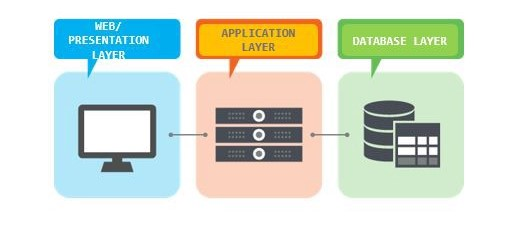
\includegraphics[width=8cm,height=3.3cm,keepaspectratio]{images/3tier}
\end{center}

This project utilises the multi-tier architecture (often referred to as n-tier architecture) platform. Multi-tier architecture or multilayered architecture is a client–server architecture in which presentation, application processing, and data management functions are physically separated. The most widespread use of multi-tier architecture is the three-tier architecture. This project consists of three main components, all working together: The web application, which represents the presentation layer, allows users to visualise various sorting algorithms, register and login, upload and view past sorts from other users. The Flask server, which represents the logic tier, handles requests such as account registration and log in, and uploading and retrieving of sorts by users. The databases: the MongoDB database which stores user details and the Firebase database which stores all previous sorts.

\begin{center}
    \includegraphics[width=15cm,height=17cm,keepaspectratio]{images/AppDesign}
\end{center}
\newpage

\section{Web Application}
The web application was designed and developed first as this is the main aspect of the project itself. The main objective of the web application was to allow a user to choose a sorting algorithm and be able to visualise it. Secondary objectives, which were developed at a later point, was to allow users to register and log in to an account, and have the ability to upload and view previous sorts. This was greatly aided by the decision to use ReactJS as discussed in Chapter 3 The web application consists of four main pages: 

\begin{itemize}
    \item \textbf{Sorting Page} - The sorting page, as shown in Figure \ref{fig:main_page}, is the main page of the application. Allows a user to choose one of several sorting algorithms to visualise, generate a random array of elements to sort, utilize the ScreenFlow API and specify their own dataset to sort.
    \item \textbf{Login Page} - The login page handles user authentication and will login a user to the application if that user exists within the database. The user will then be redirected to the sorting page, with new functionality available such as accessing the ScreenFlow API and uploading one's own dataset.
    \item \textbf{Register Page} - The register page handles user authentication and will register a user with the application. The user will then be redirected to the login page, where they can then attempt to login.
    \item \textbf{Sorts Page} - The sorts page displays all previous sorts recorded and saved by past users.
\end{itemize}

\begin{figure}[!h]
    \centering
    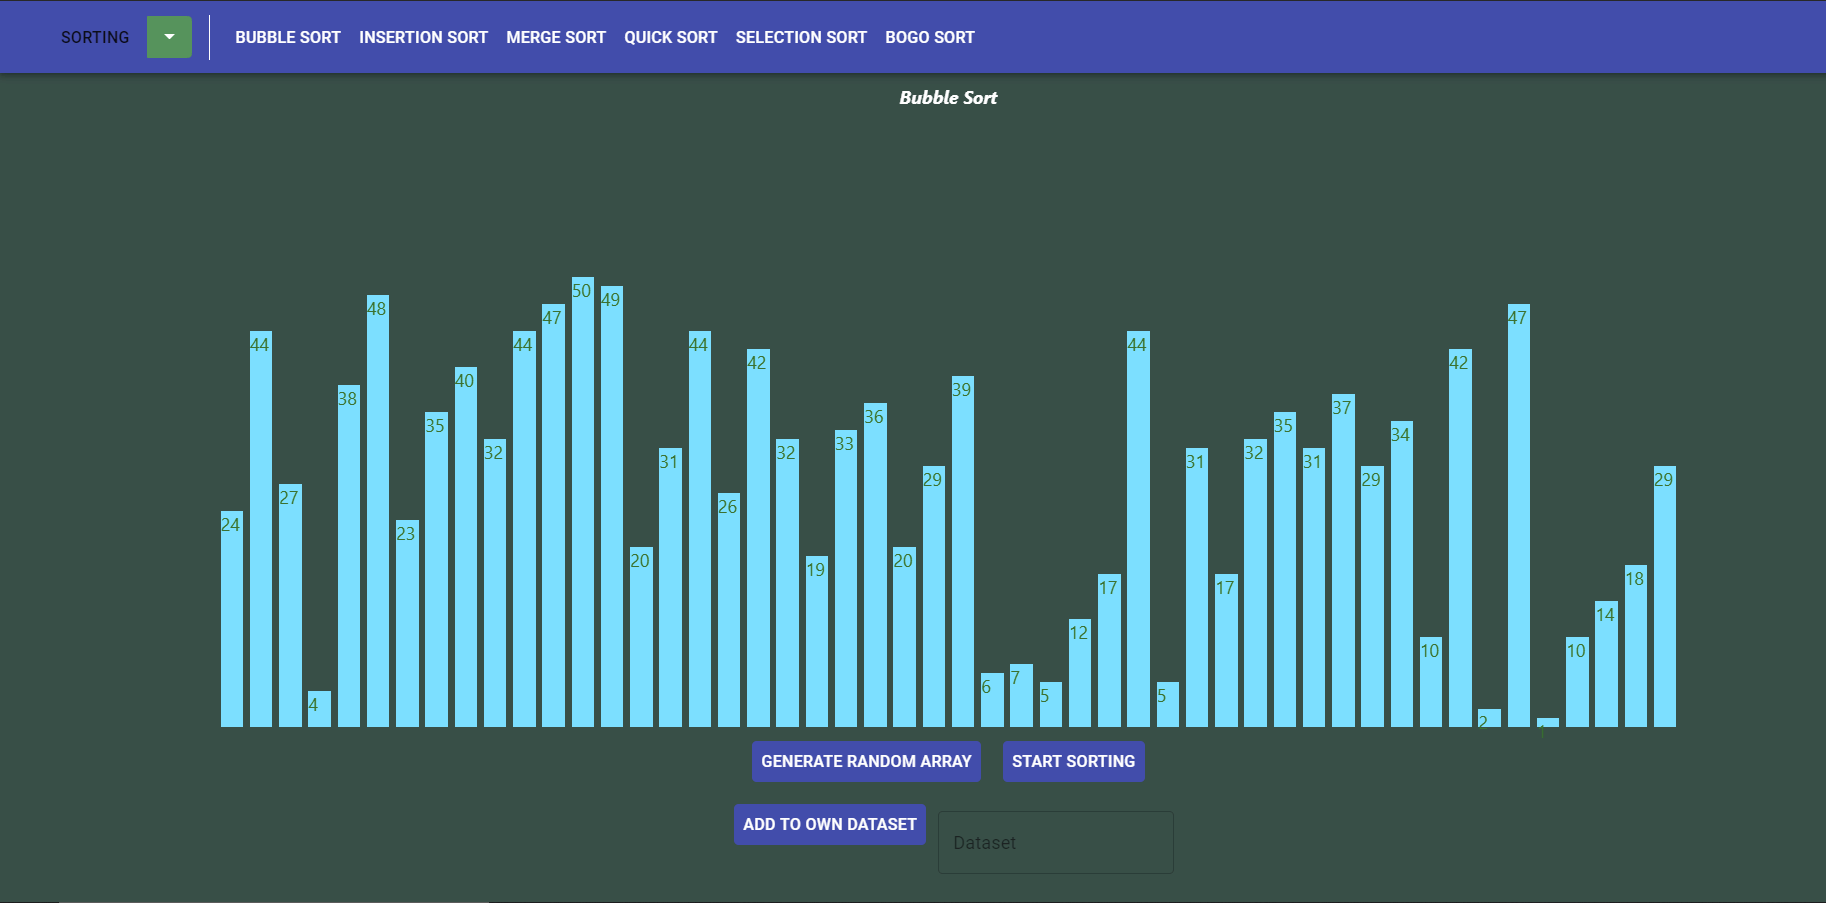
\includegraphics[scale=.35]{images/web_app_main}
    \label{fig:main_page}
\end{figure}

\subsection{Sorting}
\begin{center}
    \includegraphics[height=6.5cm,width=13cm]{images/sorting}
    \label{fig:main_page}
\end{center}
There are currently seven algorithms that can be visualised within the application. Currently, all sorting algorithms have been written using JavaScript \cite{sortalgs_guide}. They are as follows:

\begin{itemize}
    \item Bubble Sort \cite{bub_sor}
    \item Heap Sort
    \item Insertion Sort
    \item Merge Sort
    \item Quick Sort
    \item Selection Sort
    \item Shell Sort
\end{itemize}

\subsubsection{Bubble Sort}
\begin{center}
    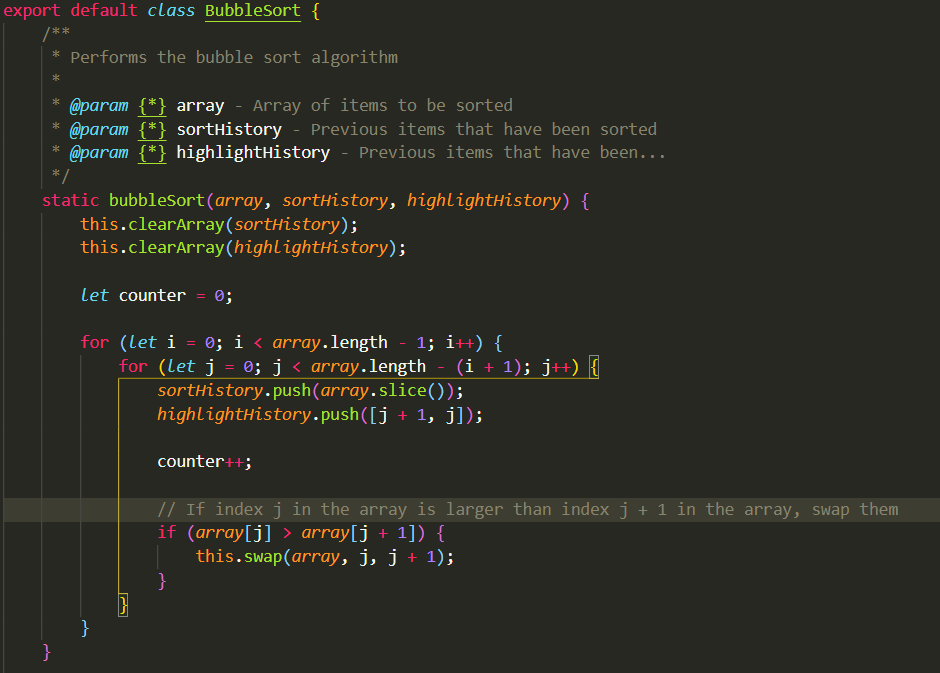
\includegraphics[width=12cm,height=15cm,keepaspectratio]{images/bubblesort}
\end{center}
Bubble sort, sometimes referred to as sinking sort, is a simple sorting algorithm that repeatedly steps through the list, compares adjacent elements and swaps them if they are in the wrong order \cite{bubble_sort}. The pass through the list is repeated until the list is sorted. The algorithm, which is a comparison sort, is named for the way smaller or larger elements "bubble" to the top of the list.
\par
\bigskip
This simple algorithm performs poorly in real world use and is used primarily as an educational tool. More efficient algorithms such as Tim Sort, or Merge Sort are used by the sorting libraries built into popular programming languages such as Python and Java.

\paragraph{How it works in the context of the application}
Bubble sort works by comparing adjacent pairs of objects in the array using nested for loops \cite{bubble_sort_geeks}. Sorted elements are pushed into \lstinline{sortedElements} as a new array object. Elements that need to be sorted are pushed into \lstinline{selectedElements}. If the objects are not in the correct ordered, they are swapped so that the largest of the two moves up.

% \subsubsection{Heap Sort}
% \begin{center}
%     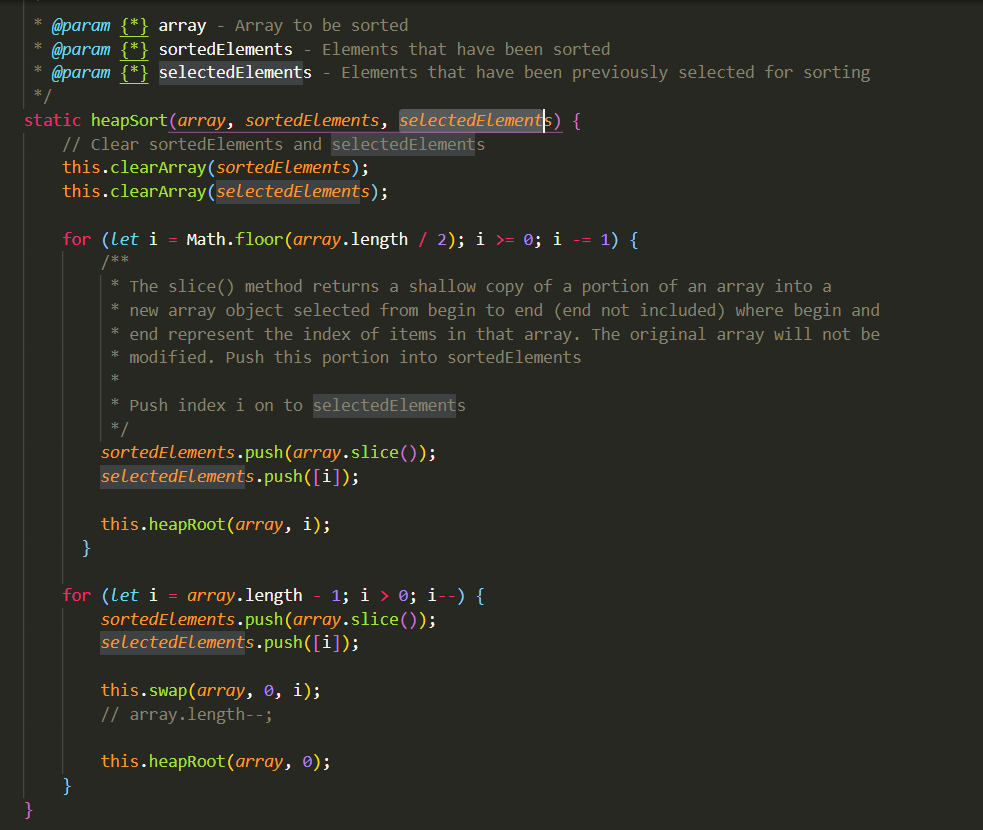
\includegraphics[width=6cm,height=8cm,keepaspectratio]{images/heapsort1}
%     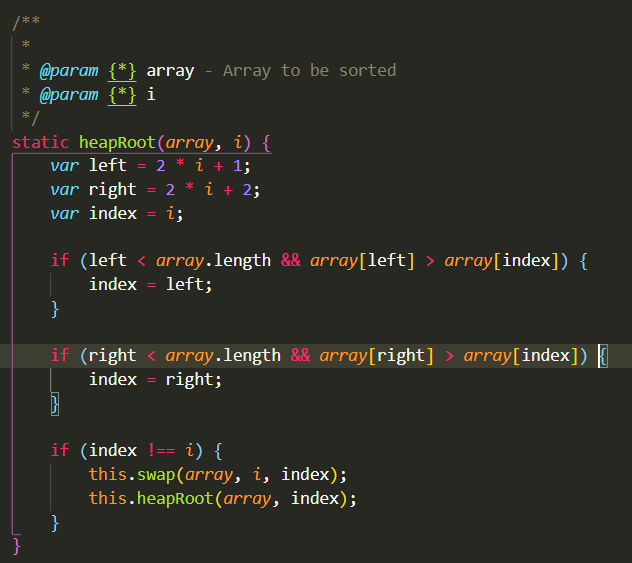
\includegraphics[width=6cm,height=8cm,keepaspectratio]{images/heapsort2}
% \end{center}
% Heap Sort is a comparison-based sorting algorithm. Heap Sort can be thought of as an improved Selection Sort: like Selection Sort, Heap Sort divides its input into a sorted and an unsorted region, and it iteratively shrinks the unsorted region by extracting the largest element from it and inserting it into the sorted region. Unlike Selection Sort, Heap Sort does not waste time with a linear-time scan of the unsorted region; rather, heap sort maintains the unsorted region in a heap data structure to more quickly find the largest element in each step.
% \par
% \bigskip
% Although somewhat slower in practice on most machines than a well-implemented Quick Sort, it has the advantage of a more favorable worst-case O(n log n) runtime. Heap Sort is an in-place algorithm, but it is not a stable sort.

% \paragraph{How it works in the context of the application}

\subsubsection{Insertion Sort}
\begin{center}
    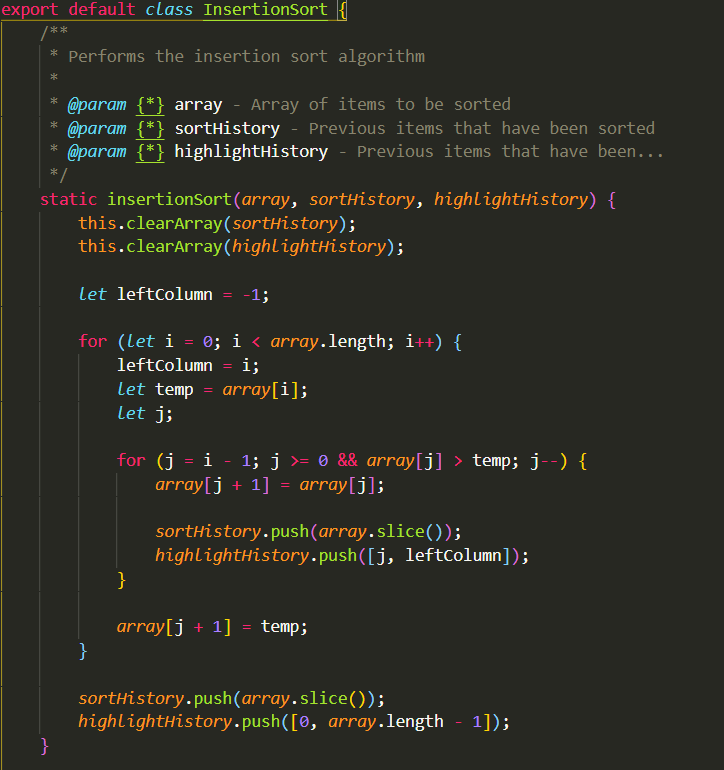
\includegraphics[width=12cm,height=15cm,keepaspectratio]{images/insertionsort}
\end{center}
Insertion sort is a simple sorting algorithm that builds the final sorted array (or list) one item at a time \cite{insertion_sort}. It is much less efficient on large lists than more advanced algorithms such as Quick Sort, Heap Sort, or Merge Sort. However, insertion sort provides several advantages:

\begin{itemize}
    \item \textbf{Efficient} - Efficient for (quite) small data sets, much like other quadratic sorting algorithms
    \item \textbf{Stable} - Does not change the relative order of elements with equal keys
    \item \textbf{Online} - Can sort a list as it receives it
    \item \textbf{Adaptive} - Efficient for data sets that are already substantially sorted:
\end{itemize}

When people manually sort cards in a bridge hand, most use a method that is similar to insertion sort.

\paragraph{How it works in the context of the application}
Insertion sort iterates, consuming one input element each repetition, and growing a sorted output list \cite{insertion_sort_geeks}. At each iteration, insertion sort removes one element from the input data, finds the location it belongs within the sorted list, and inserts it there. It repeats until no input elements remain.

\subsubsection{Merge Sort}
\begin{center}
    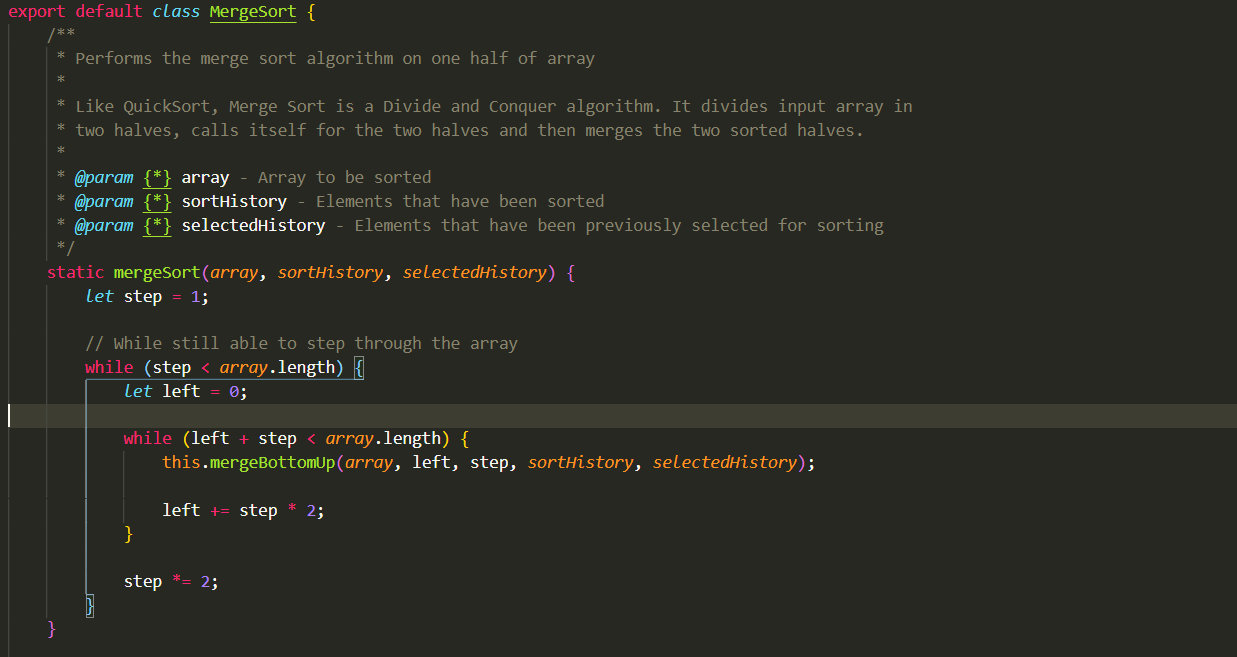
\includegraphics[width=12cm,height=6cm,keepaspectratio]{images/mergesort1}
    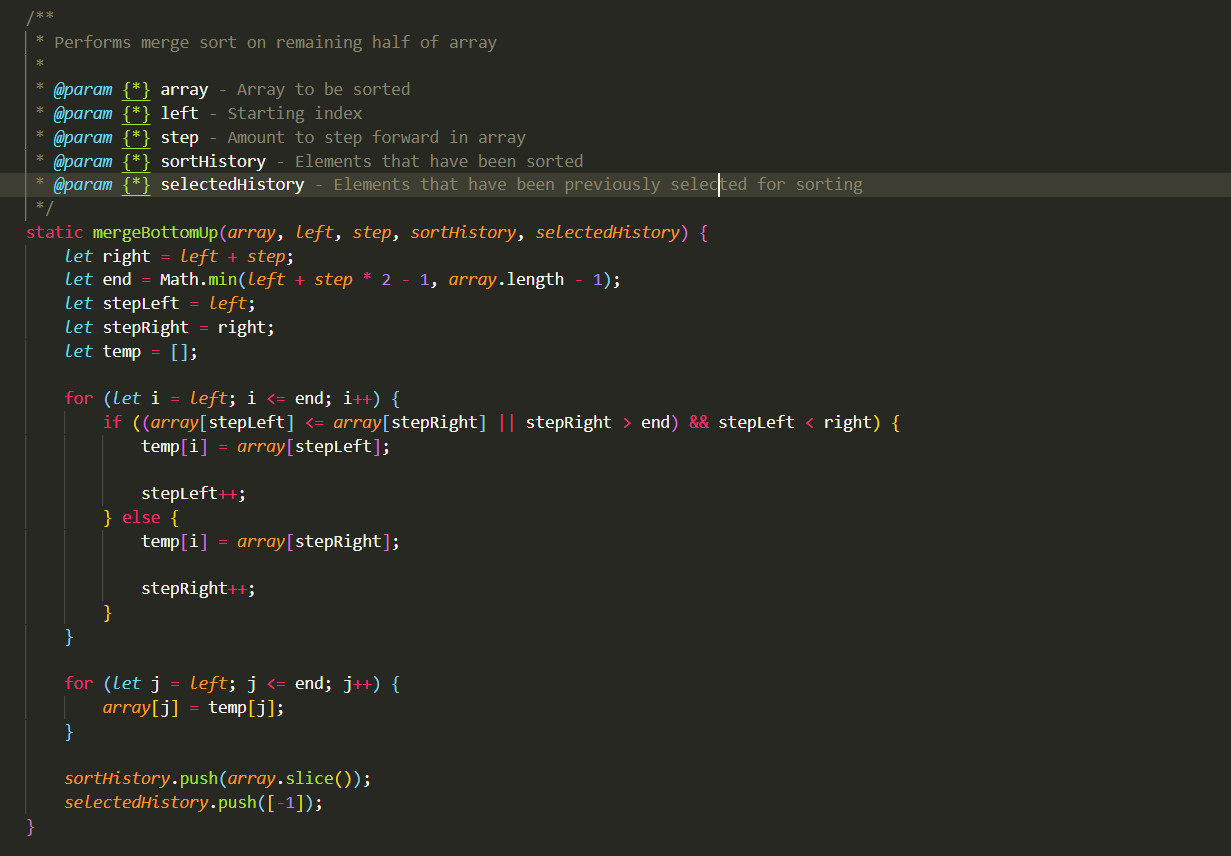
\includegraphics[width=12cm,height=6cm,keepaspectratio]{images/mergesort2}
\end{center}
Merge Sort is an efficient, general-purpose, comparison-based sorting algorithm \cite{merge_sort}. Most implementations produce a stable sort, which means that the order of equal elements is the same in the input and output. It divides input array in two halves, calls itself for the two halves and then merges the two sorted halves.

\paragraph{How it works in the context of the application}
A middle point is found and the array is divided in two halves. The sub-arrays are then recursively sorted in each of the two sub-problems created by the divide step. That is, recursively sort the sub-array \lstinline{array[p..q]} and recursively sort the sub-array \lstinline{array[q+1..r]}. The two sorted sub-arrays are then merged back into a single sorted array \cite{merge_sort_geeks}.

\subsubsection{Quick Sort}
\begin{center}
    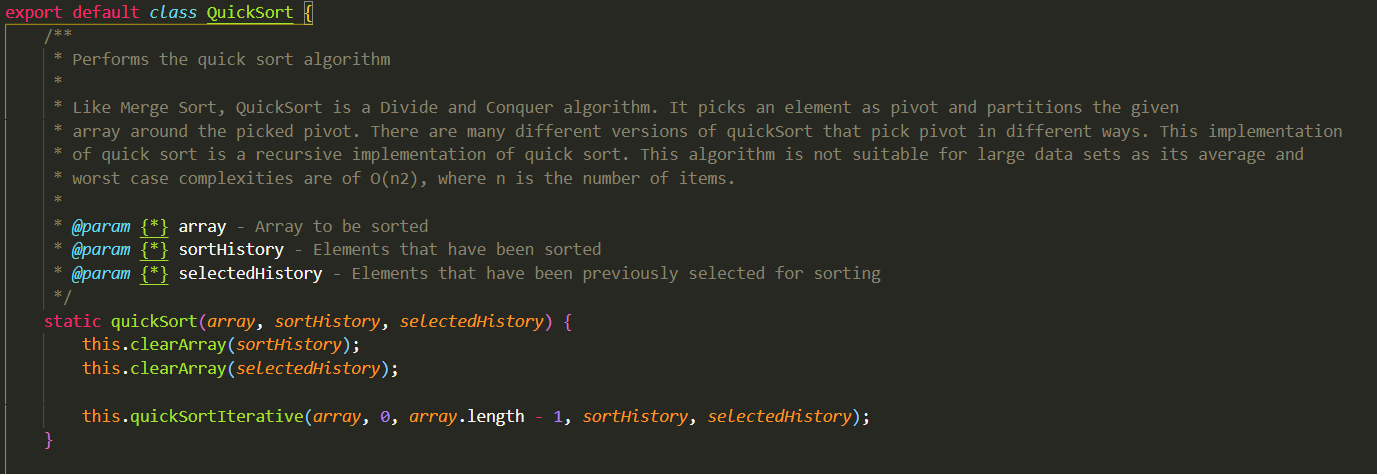
\includegraphics[width=12cm,height=12cm,keepaspectratio]{images/quicksort1}
    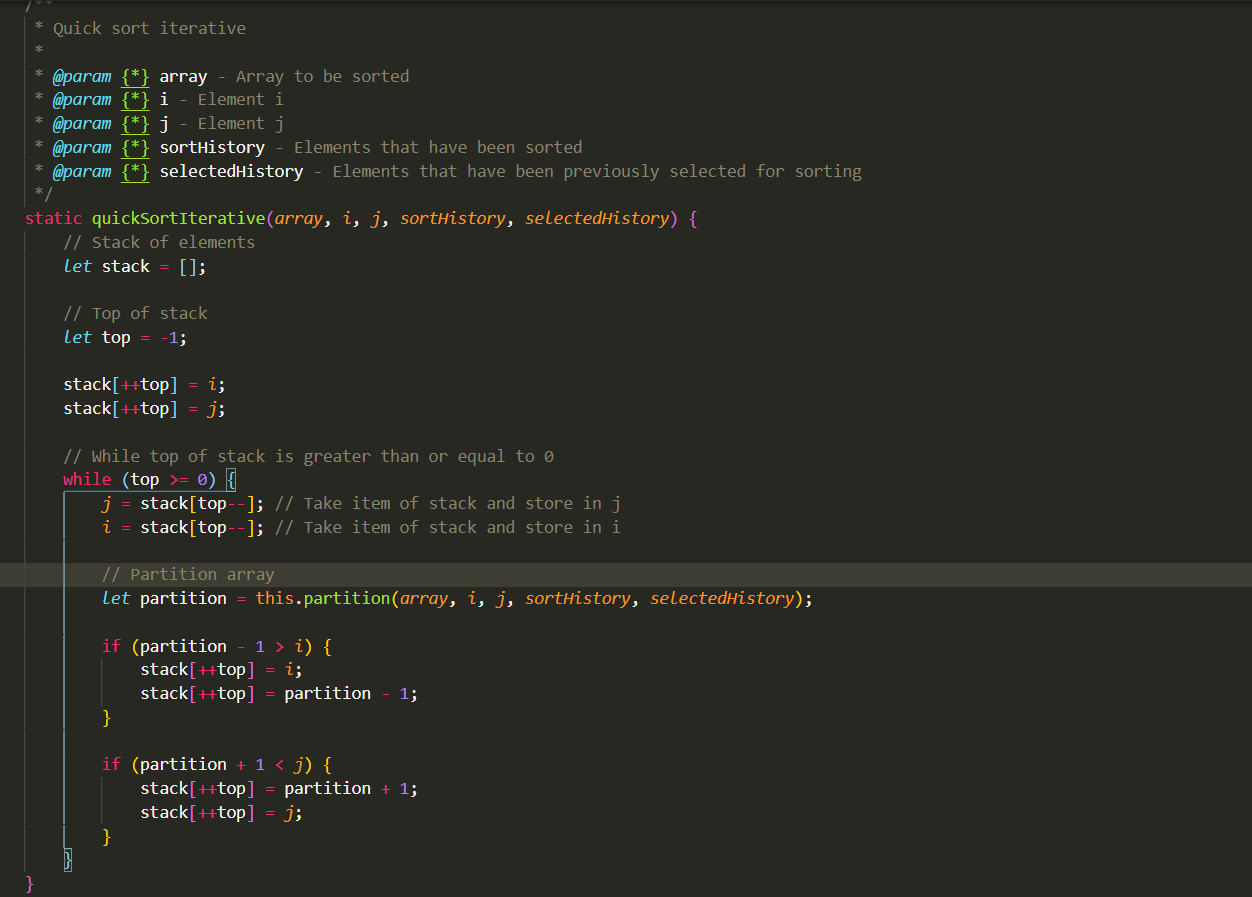
\includegraphics[width=12cm,height=12cm,keepaspectratio]{images/quicksort3}
    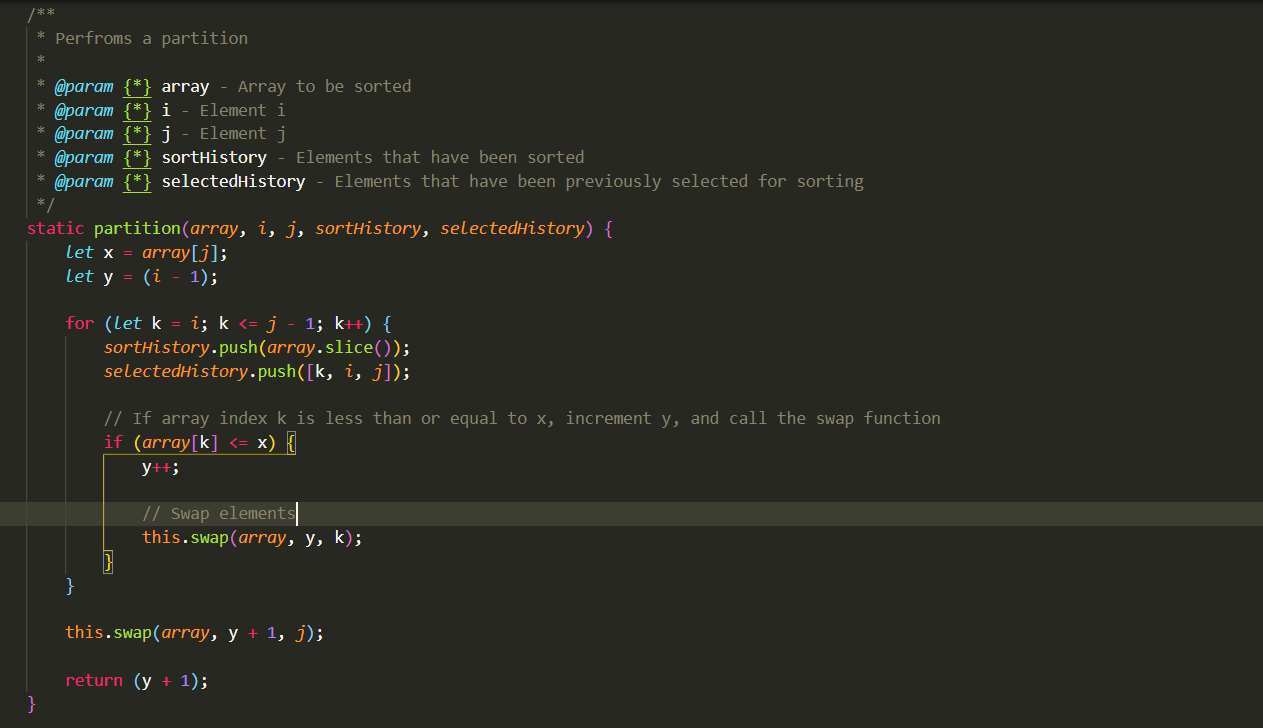
\includegraphics[width=12cm,height=12cm,keepaspectratio]{images/quicksort2}
\end{center}
Quick Sort is an efficient sorting algorithm \cite{quick_sort}.
Quick Sort is a divide-and-conquer algorithm. It works by selecting a 'pivot' element from the array and partitioning the other elements into two sub-arrays, according to whether they are less than or greater than the pivot. The sub-arrays are then sorted recursively. This can be done in-place, requiring small additional amounts of memory to perform the sorting.
\par
\bigskip
Quick Sort is a comparison sort, meaning that it can sort items of any type for which a "less-than" relation (formally, a total order) is defined. Efficient implementations of Quick Sort are not a stable sort, meaning that the relative order of equal sort items is not preserved.
\par
\bigskip
Mathematical analysis of Quick Sort shows that, on average, the algorithm takes O(n log n) comparisons to sort n items. In the worst case, it makes O(n2) comparisons, though this behavior is rare.

\paragraph{How it works in the context of the application}
A “pivot” item is found in the array. A left and right pointer is started in the first and last item in the array, respectively. While the value at the left pointer in the array is less than the pivot value, move the left pointer to the right (add 1). This continues until the value at the left pointer is greater than or equal to the pivot value. While the value at the right pointer in the array is greater than the pivot value, move the right pointer to the left (subtract 1). This continues until the value at the right pointer is less than or equal to the pivot value. If the left pointer is less than or equal to the right pointer, the values at these locations in the array are swapped. The left pointer  is moved to the right by one and the right pointer is moved to the left by one. If the left pointer and right pointer don’t meet, the process is started again \cite{quick_sort_geeks}.

\subsubsection{Selection Sort}
\begin{center}
    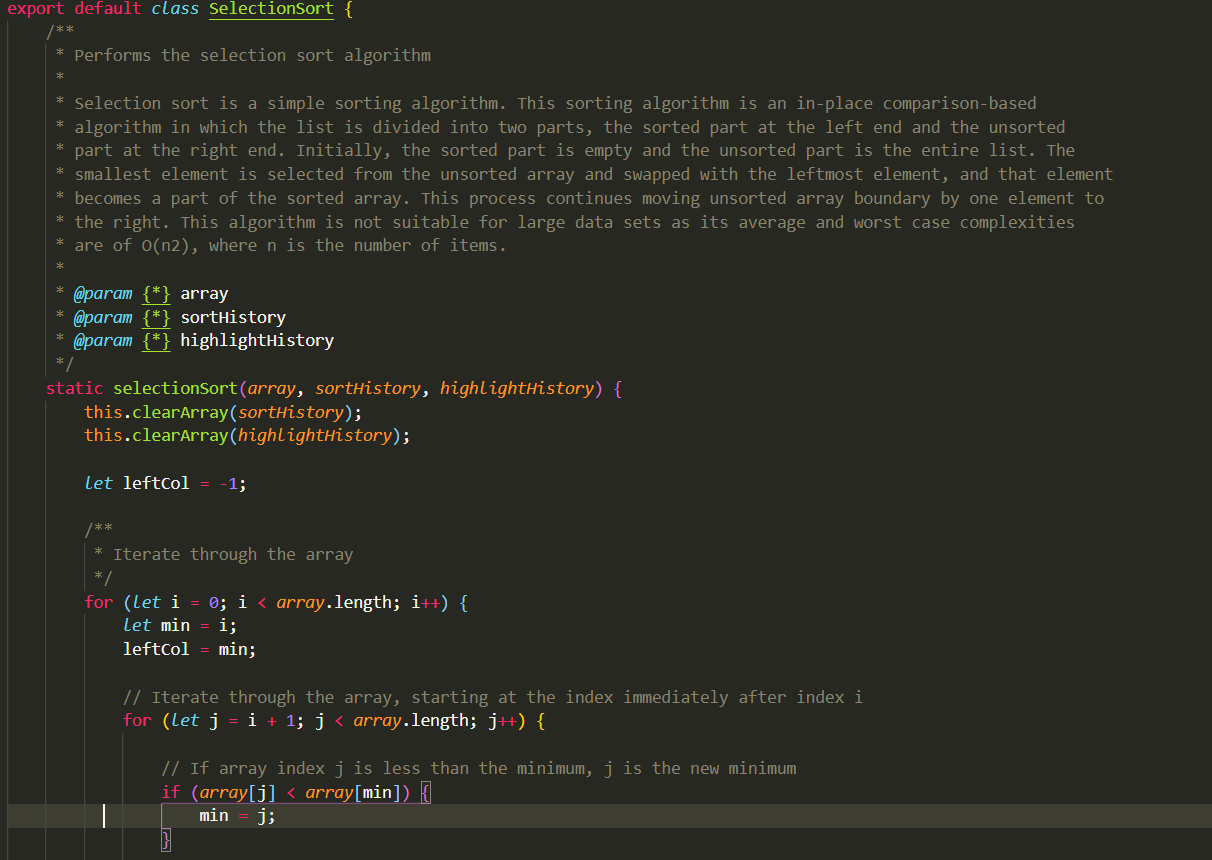
\includegraphics[width=12cm,height=15cm,keepaspectratio]{images/selectionsort1}
    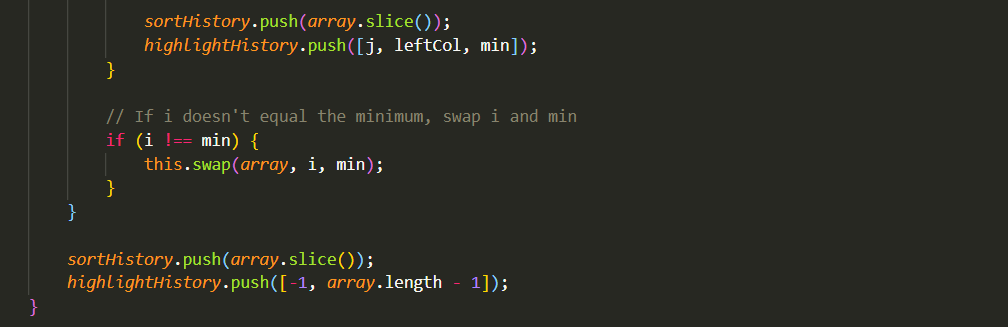
\includegraphics[width=12cm,height=15cm,keepaspectratio]{images/selectionsort2}
\end{center}
Selection sort is an in-place comparison sorting algorithm \cite{selection_sort}. It has an O(n2) time complexity, which makes it inefficient on large lists, and generally performs worse than the similar insertion sort. Selection sort is noted for its simplicity and has performance advantages over more complicated algorithms in certain situations, particularly where auxiliary memory is limited.
\par
\bigskip
The algorithm divides the input list into two parts: a sorted sublist of items which is built up from left to right at the front (left) of the list and a sublist of the remaining unsorted items that occupy the rest of the list. Initially, the sorted sublist is empty and the unsorted sublist is the entire input list. The algorithm proceeds by finding the smallest (or largest, depending on sorting order) element in the unsorted sublist, exchanging (swapping) it with the leftmost unsorted element (putting it in sorted order), and moving the sublist boundaries one element to the right.
\par
\bigskip
The time efficiency of selection sort is quadratic, so there are a number of sorting techniques which have better time complexity than selection sort. One thing which distinguishes selection sort from other sorting algorithms is that it makes the minimum possible number of swaps, n − 1 in the worst case.

\paragraph{How it works in the context of the application}
For the first position in the sorted list, the whole list is scanned sequentially. The whole array is sorted to find the lowest value. After one iteration, the minimum value is stored in the first position of the sorted list. For the second position, the rest of the list is scanned in a linear manner. The same process is applied to the rest of the items in the array \cite{selection_sort_geeks}.

\subsubsection{Shell Sort}
\begin{center}
    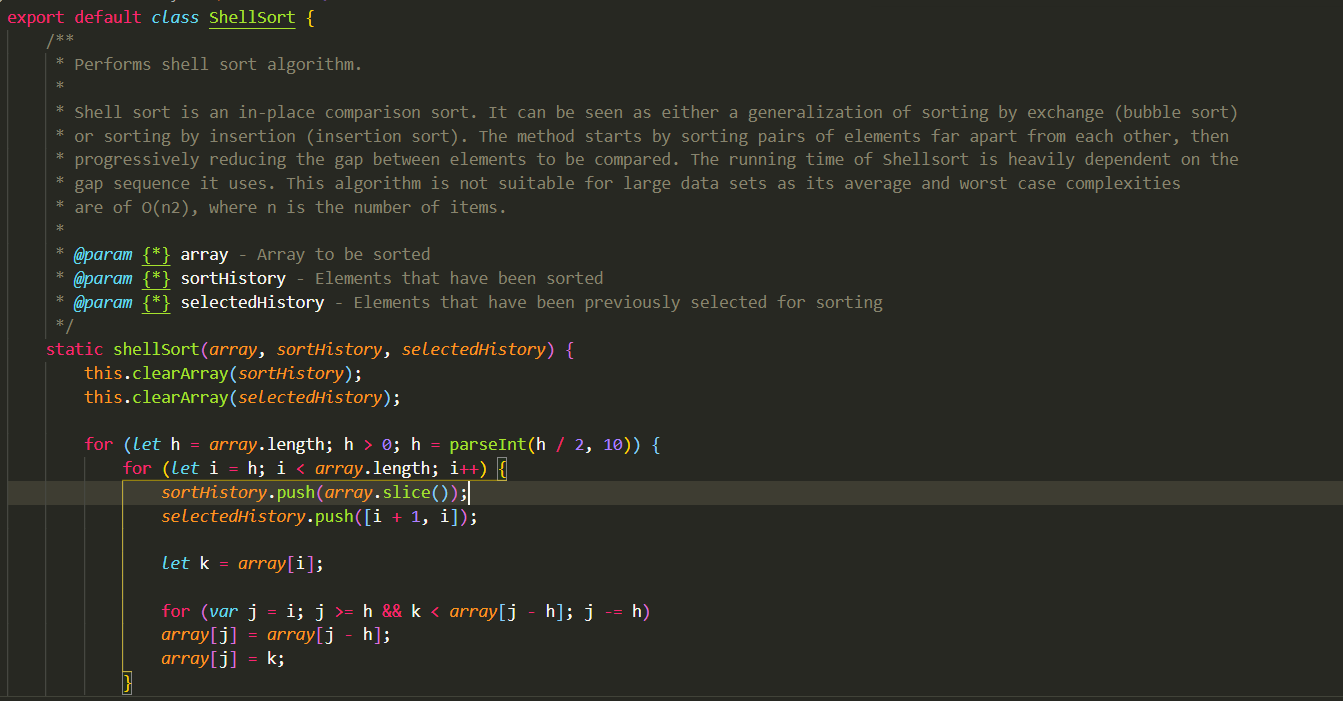
\includegraphics[width=12cm,height=8cm,keepaspectratio]{images/shellsort}
\end{center}
Shell Sort is an in-place comparison sort \cite{shell_sort}. It can be seen as either a generalization of sorting by exchange (bubble sort) or sorting by insertion (insertion sort). The method starts by sorting pairs of elements far apart from each other, then progressively reducing the gap between elements to be compared. Starting with far apart elements, it can move some out-of-place elements into position faster than a simple nearest neighbor exchange. The running time of Shell Sort is heavily dependent on the gap sequence it uses. For many practical variants, determining their time complexity remains an open problem.
\par
\bigskip

\paragraph{How it works in the context of the application}
The idea of Shell Sort is to allow exchange of far items. In Shell Sort, we make the array h-sorted for a large value of h. We keep reducing the value of h until it becomes 1. An array is said to be h-sorted if all sublists of every h’th element is sorted \cite{shell_sort_geeks}.
\par
\bigskip
Bogo Sort and Heap Sort have been programmed as well, however, they are not fully working as of now and as such, they are not covered in this section.

\subsection{Visualization}
\begin{center}
    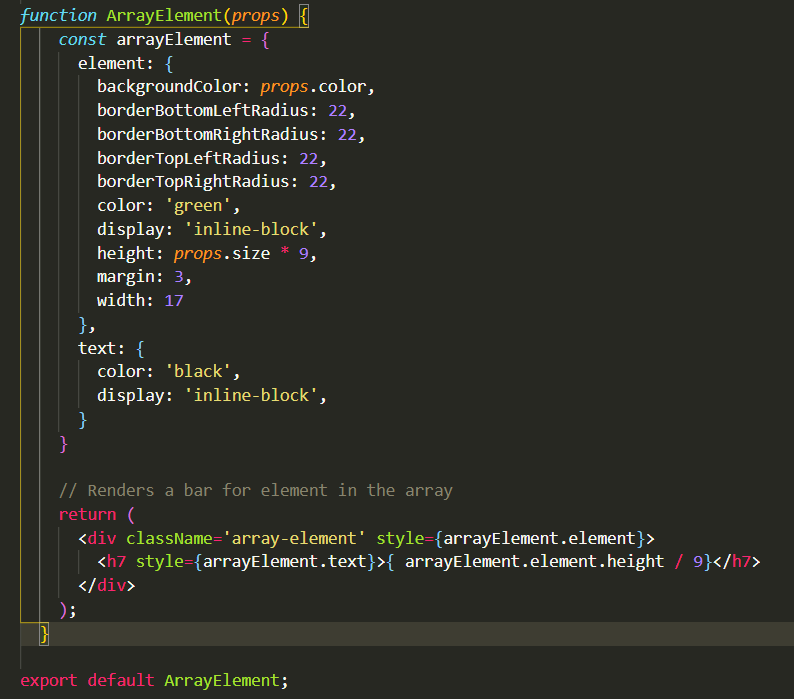
\includegraphics[height=8cm,width=12cm]{images/arrayelement}
    
\includegraphics[height=1cm,width=12cm]{images/maparray}
\end{center}
The ArrayElement renders a bar that will represent each element in the array. In MainPage, each element and it's index will be mapped and then visually represented by the bar generated using ArrayElement \cite{react_bar}.

\newpage
\section{Flask Server}
The Flask server, which is hosted on PythonAnywhere, is the middle-man of the entire application and allows the web application to communicate with the database. The server was developed and integrated into the web application secondly alongside the database. It handles requests, such as user login requests, user registration requests, uploading saved sorts, etc. made by the web application and performs the appropriate action. The database is then read and/or updated based on this. 

\begin{center}
    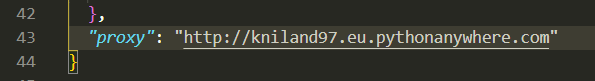
\includegraphics[width=12cm,height=10cm,keepaspectratio]{images/proxy}
\end{center}

\section{Databases}
This application utilizes two databases: a MongoDB database, which is used to store user details and a Firebase database, which stores all previous sorts.

\subsection{MongoDB}
MongoDB was chosen as the database to store user details as MongoDB stores data records as BSON documents. BSON is a binary representation of JSON documents, though it contains more data types than JSON. I thought this would be the best way to save user details since there are several libraries, such as bcrypt, that could work hand-in-hand. The value of a field can be any of the BSON data types, including other documents, arrays, and arrays of documents. 

\begin{center}
    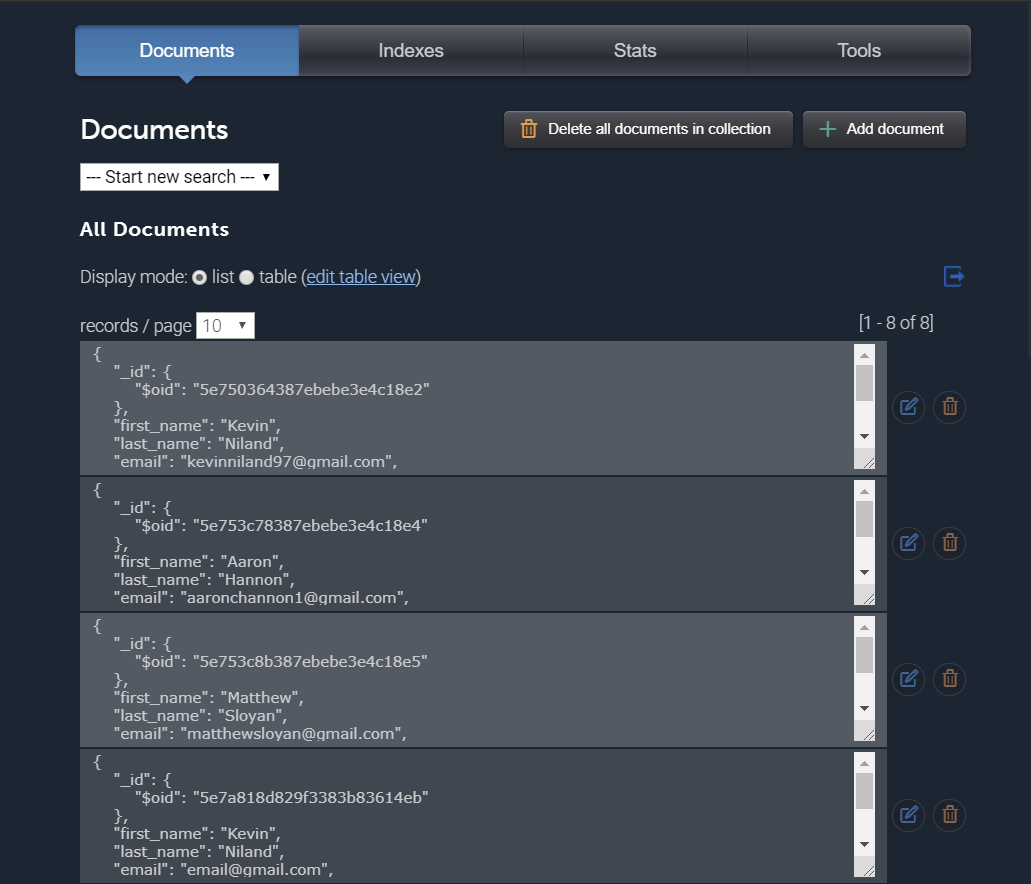
\includegraphics[width=12cm,height=6cm,keepaspectratio]{images/mlab}
\end{center}

\newpage
\subsection{Firebase}
Firebase was chosen as the database to store previous sorts as it provides an easy and simple way to store files. There are a number of React libraries, such as React File Uploader, that have been specifically developed to work with Firebase which provides a simple and easy way to upload a file to Firebase. Firebase itself also provides a number of methods, such as getMetadata() which will retrieve the file type and getDownloadURL() which will retrieve the download URL for each file, that enable an application to retrieve these files easily.

\begin{center}
    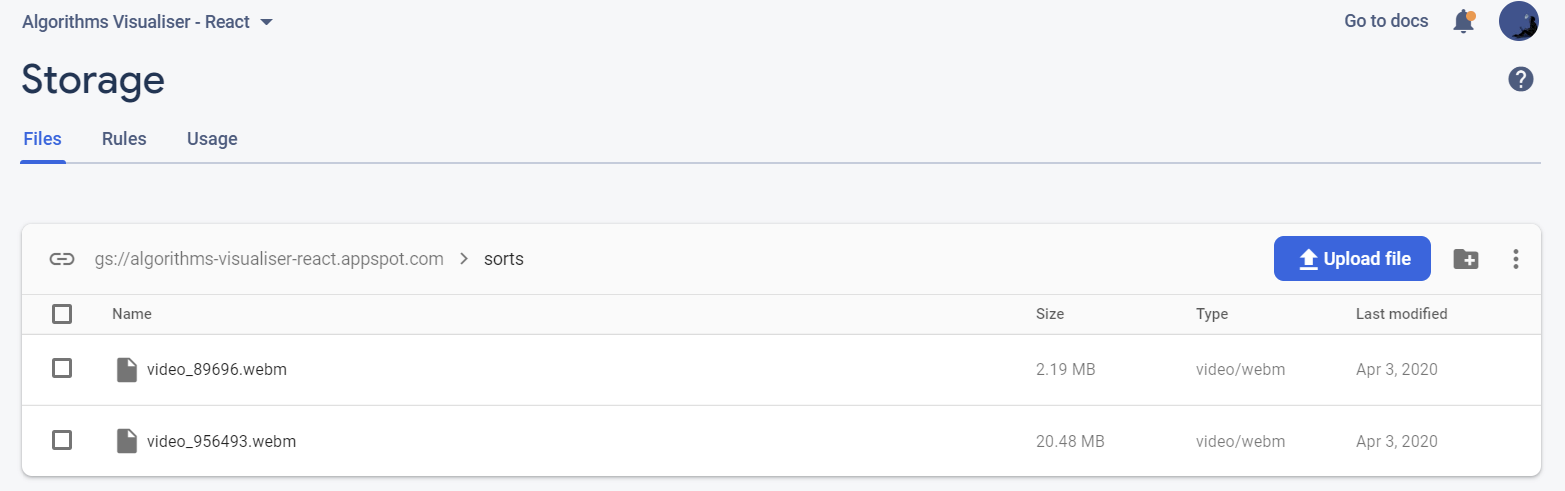
\includegraphics[width=12cm,height=15cm,keepaspectratio]{images/firestore}
\end{center}

Firebase Storage was designed specifically to allow users to upload files, such as images and videos. Data is stored in a Google Cloud Storage bucket, an exabyte scale object storage solution with high availability and global redundancy.
\chapter{System Evaluation}
This chapter evaluates the system, analysing the various aspects of the project 
to ensure the requirements of the project were met and discusses the various 
types of testing that was performed throughout the software development cycle to
ensure each of the requirements was met and the software was of high quality. 

\section{Overview}
The system was designed and developed using the Test Driven Development (TDD) 
methodology. As each unit of code was written and before each new component was 
integrated into the system, appropriate tests were carried out and adjusted if 
needed. Because of this, a lot of bugs were caught early on, allowing them to be
fixed with minimal disruption to the system as a whole. This also allowed the 
system to be redesigned early on when necessary.

\par
\bigskip
The types of testing carried out were as follows:

\begin{itemize}
    \item End-to-End Testing
    \item Exploratory Testing
    \item Functional Testing
    \item Graphical User Interface (GUI) Testing
    \item Integration Testing
    \item Unit Testing
    \item System Testing
\end{itemize}

\section{End-to-End Testing}
\begin{center}
    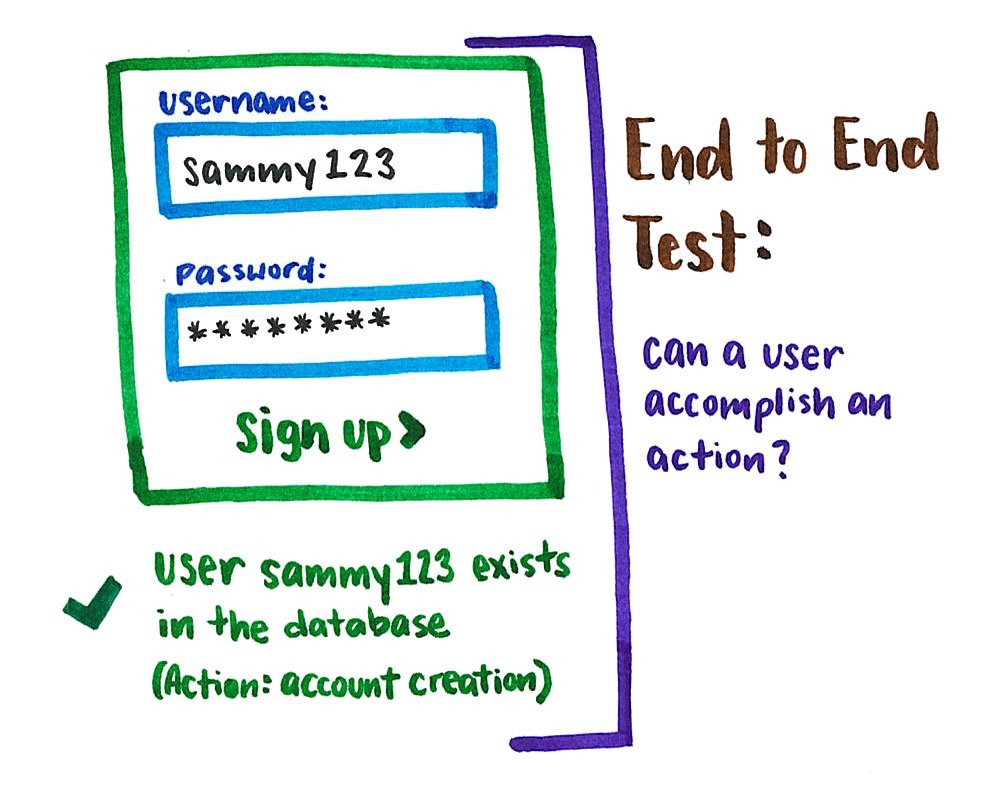
\includegraphics[width=6cm,height=10cm,keepaspectratio]{images/e2e_1}
    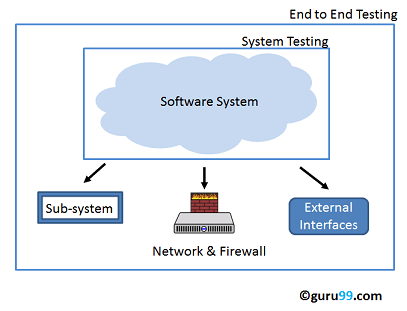
\includegraphics[width=6cm,height=10cm,keepaspectratio]{images/e2e_2}
\end{center}

End-to-end testing is a technique used to test whether the flow of an 
application right from start to finish is behaving as expected. The purpose of 
performing end-to-end testing is to identify system dependencies and to ensure
that the data integrity is maintained between various system components and 
systems.
\par
\bigskip
The entire application is tested for critical functionalities such as 
communicating with the other systems, interfaces, database, network, and other 
applications. This type of testing was carried out at the end, when all features were fully implemented. To perform 'test cases', the system was used in a way that a user would typically use the system. All features were tested to see if the appropriate behaviour happened, such as visualizing an algorithm, registering for an account, logging into an account, recording a sort, uploading a sort, and viewing past sorts.

\section{Exploratory Testing}
\begin{center}
    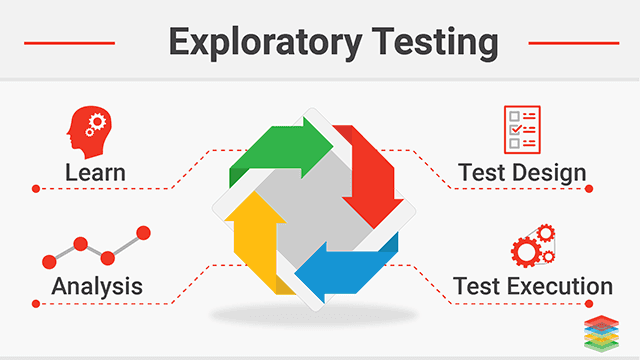
\includegraphics[width=12cm,height=10cm,keepaspectratio]{images/xenonstack-what-is-exploratory-testing}
\end{center}
Exploratory testing is a technique or a method whose aim is to discover the
flaws during the process of software development. Exploratory Testing is widely used in Agile models and is all about discovery, investigation, and learning. It emphasizes personal freedom and responsibility of the individual tester.

\par
\bigskip

This technique of testing is concerned about the qualitative assurance of the 
software. It is used to discover the anonymous issues during the process of 
development of software. Exploratory testing was carried out throughout development and helped prevent massive system flaws from remaining in the application and causing other bugs and/or having to fix these issues down the line, where it mightn't be possible to fix them or having to perform a complete overhaul of the system. One such flaw was in regards to an early design. Initially, there would be a 'master' navigation bar, with each of the application's pages appearing and being able to be navigated to from here. This caused the visualization aspect to not work properly, as the user would not be able to select an algorithm to visualize. This resulted in the system being redesigned to what it is now.

\section{Functional Testing}
\begin{center}
    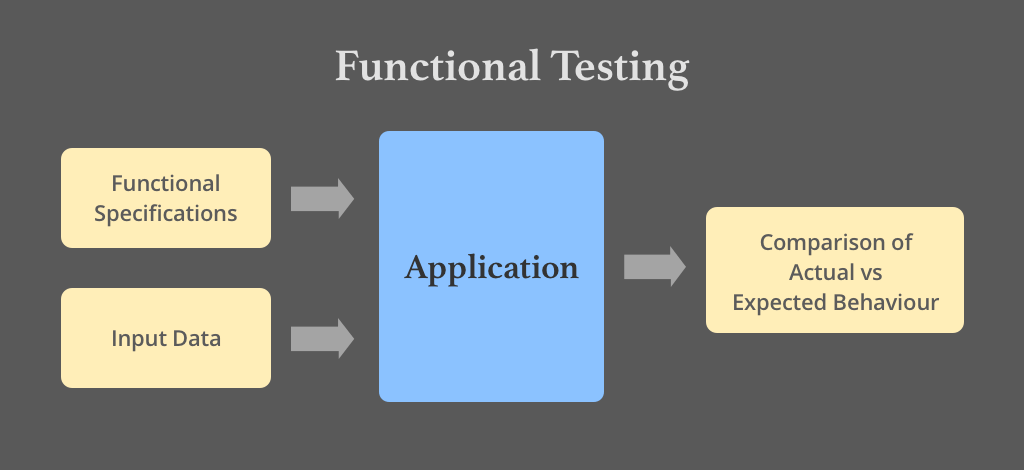
\includegraphics[width=12cm,height=10cm,keepaspectratio]{images/Functional-Testing-feature-image}
\end{center}
Functional Testing is a type of software testing whereby the system is tested 
against the functional requirements/specifications.
\par
\bigskip
Functions (or features) are tested by feeding them input and examining the 
output. Functional testing ensures that the requirements are properly satisfied 
by the application. This type of testing is not concerned with how processing 
occurs, but rather, with the results of processing. It simulates actual system 
usage but does not make any system structure assumptions.
\par
\bigskip
During functional testing, Black Box Testing technique is used in which the 
internal logic of the system being tested is not known to the tester.

\subsection{Web Application}


\section{Graphical User Interface (GUI) Testing}
\begin{center}
    
\includegraphics[width=12cm,height=10cm,keepaspectratio]{images/gui_testing}
\end{center}
Graphical User Interface (GUI) Testing is a software testing type that checks
the Graphical User Interface of the application under test. GUI testing involves
checking the screens with the controls like menus, buttons, icons, and all types
of bars - toolbar, menu bar, dialog boxes, and windows, etc. The purpose of GUI 
Testing is to ensure UI functionality works as per the specification. 
\par
\bigskip
This type of testing, like exploratory testing, was carried out in conjunction with development and as such, aided in discovering bugs with the system. As discussed above, the system needed to be redesigned due a bug discovered, which GUI testing aided in as it was discovered in a previous design that the user was not able to visualize an algorithm due to an unresponsive GUI.

\section{Integration Testing}
\begin{center}
    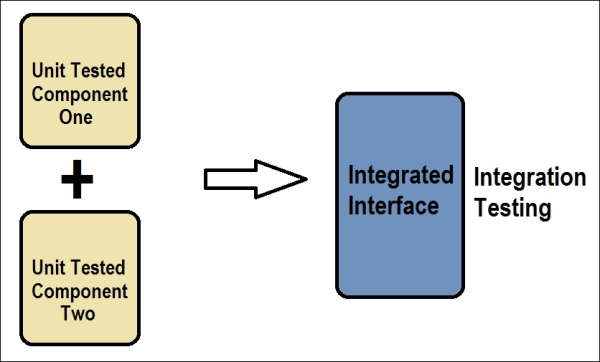
\includegraphics[width=12cm,height=10cm,keepaspectratio]{images/integration}
\end{center}
Integration testing (sometimes called integration and testing, abbreviated I&T) 
is the phase in software testing in which individual software modules are 
combined and tested as a group. Integration testing is conducted to evaluate the
compliance of a system or component with specified functional requirements.
\par
\bigskip
Integration testing was carried out throughout development and was integral in ensuring components worked with already integrated components without breaking the system. When a new component was added to the application, the entire application was tested in full before committing the changes to GitHub to make sure the new component didn't negatively affect or break the application. 

\section{Unit Testing}
\begin{center}
    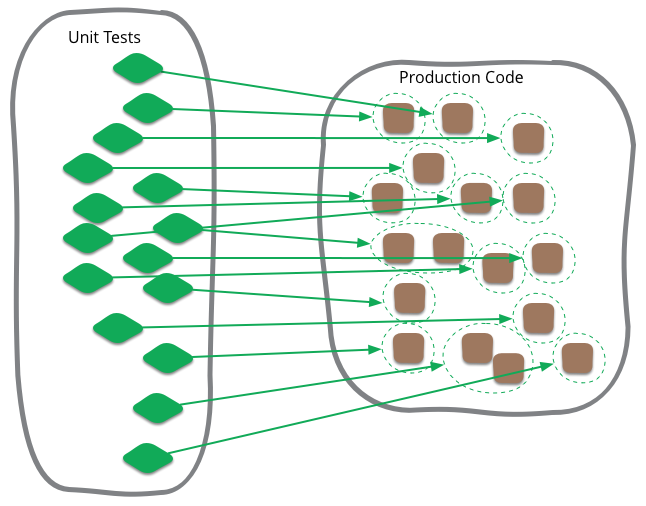
\includegraphics[width=12cm,height=8cm,keepaspectratio]{images/unit}
\end{center}
Unit Testing is a level of software testing where individual units/components
of a software are tested. The purpose is to validate that each unit of the
software performs as designed. A unit is the smallest testable part of any 
software. It usually has one or a few inputs and usually a single output.
\par
\bigskip
Unit testing was carried out on individual components before they were integrated into the system. Several different pieces of software were used to help test the application.

\subsection{Postman}
\begin{center}
    
\includegraphics[width=12cm,height=4cm,keepaspectratio]{images/postman}
\end{center}
To test the user authentication aspect of the application, Postman was used to test requests made to the database to see if a user could successfully register for an account and log into an account. Requests could be made to the database via the Flask Server (hosted on PythonAnywhere), which would then return a response.

\subsubsection{Register}
\begin{center}
    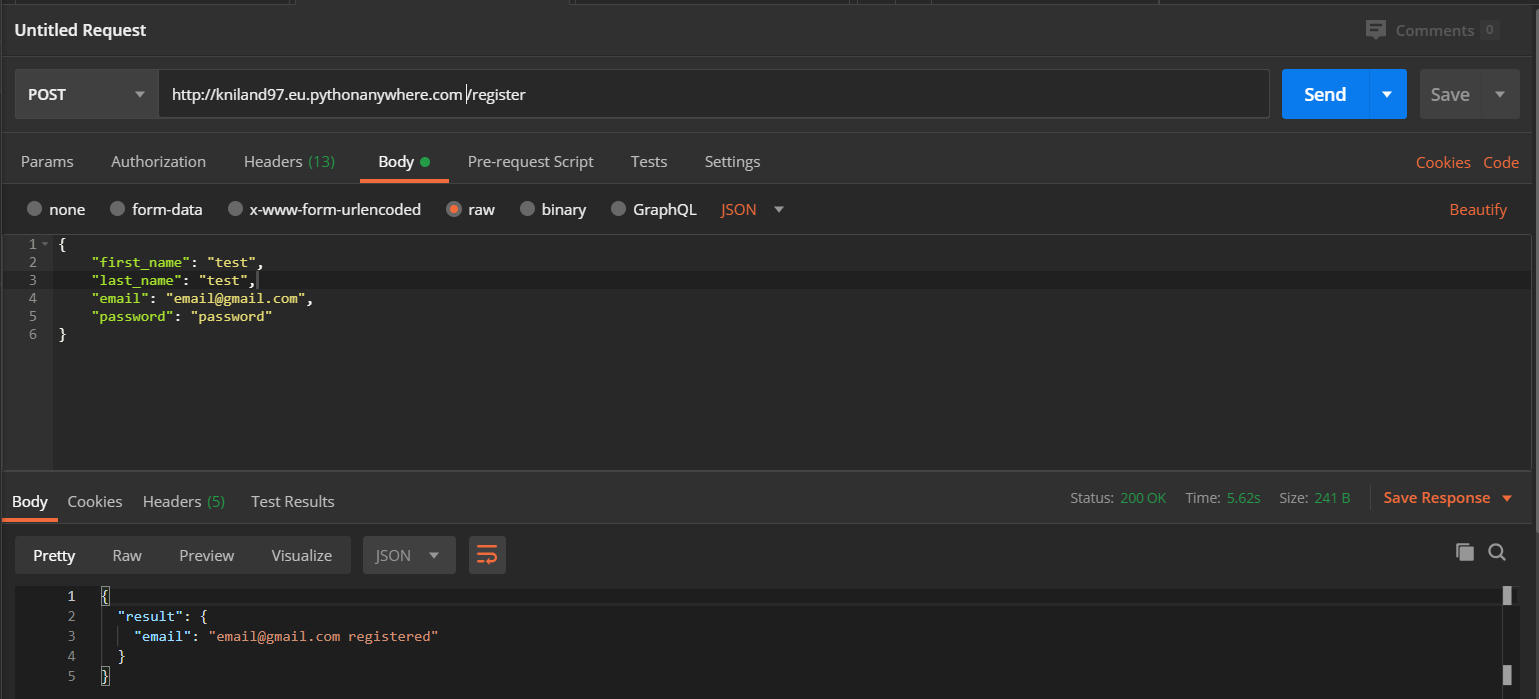
\includegraphics[width=12cm,height=4cm,keepaspectratio]{images/postman_register}
\end{center}
Using the POST method, a request is made to see if a user with the above details is able to successfully register an account with the application.

\subsubsection{Login}
\begin{center}
    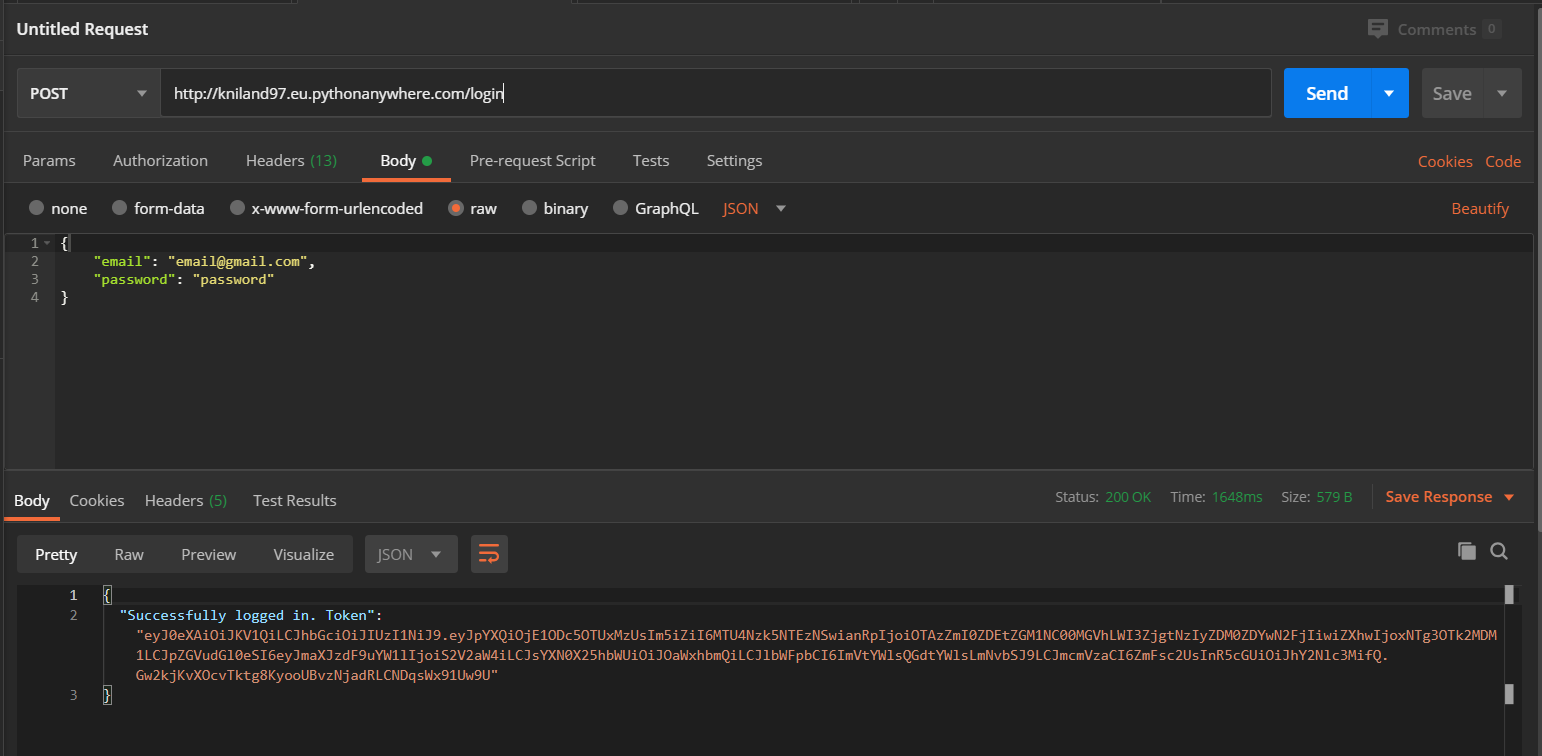
\includegraphics[width=12cm,height=4cm,keepaspectratio]{images/postman_login}
\end{center}
Using the POST method, a request is made to see if a user with the above details is able to successfully login to the application.

\subsection{Sorting Algorithms}
Before each sorting algorithm was implemented and added into the application, they were first written and tested on sample inputs and arrays.

\section{System Testing}
\begin{center}
    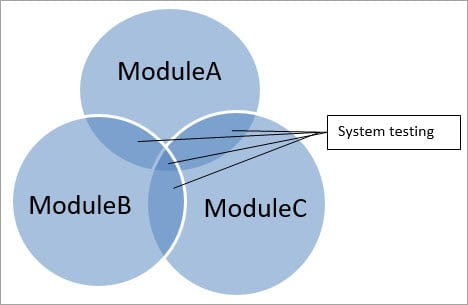
\includegraphics[width=12cm,height=10cm,keepaspectratio]{images/system-testing-example}
\end{center}
System Testing is a level of testing that validates the complete and fully
integrated software product. The purpose of a system test is to evaluate the 
end-to-end system specifications. Usually, the software is only one element of a
larger computer-based system. Ultimately, the software is interfaced with other 
software/hardware systems.
\chapter{Conclusion}
This chapter serves as a conclusion to the project. In it, the objectives of the project are analysed again briefly to evaluate whether or not they were met. It also analyses any improvements and/or changes that could be added/made to the project if it was to be developed again.

\section{Objectives}
One of the objectives of this project was to make an application that had the capabilities to visualize several different sorting algorithms, from start to finish. This application is intended and can be useful in an educational context, where users can use it to see how the programmed algorithms perform a sort of a provided array of elements. This was achieved by highlighting the elements currently chosen to be sorted and repeating this until the entire array is sorted. 
\par
\bigskip
Another one of the objectives of the project was to provide users of a system with the ability to register for an account, log in, and have the ability to access a screen record API and have the ability to upload the recording of the sort to a database, which can then be viewed by all users. The user registration/log-in system was achieved through a combination of Python and MongoDB. Creating a screen recording was done through the use of an external API, Screen Flow. Firebase was subsequently used to store these screen recordings.

\section{Reflection}
Overall, the objectives of the project were met and done to a standard that I was happy with. However, as with all software projects, there would be things I would do differently, incorporate different technologies to make a certain feature more robust, etc.

\subsection{Downfalls and Improvements}
If the project was to be repeated, a number of changes and improvements could be made. While user authentication does play a role, this could be further enhanced in several different ways such as further enhancing the viewing of all sorts aspect of the project. The user could have the option of uploading a dataset in addition to uploading a saved sort. The uploading of sorts could have been done in a better way. For instance, the Screen Record API used could have been integrated with the application more. This was attempted but due to the way the API was programmed, it does not seem like integrating it with this application in a more cohesive manner was possible at the time. 
\bigskip

Another improvement could have been to include more sorting algorithms. The application could also have shown a visualization of the code itself. For example, when a certain sorting algorithm is picked, a window would appear with the appropriate code for the selected sorting algorithm. When the array of elements is being sorted, the appropriate logic in the code could be highlighted (such as the logic for swapping elements, comparison of different elements, etc.).
\bigskip

A downfall of the application could be the user is unable to randomly generate an array of a certain size. The user is also unable to control the speed of the sort itself.

\subsection{Additions}
As this is application that visualizes algorithms, a viable addition to the application could be to incorporate pathfinding algorithms. Pathfinding algorithms were recently covered on the course in the Artificial Intelligence module. This would come with it's own challenges, however...

\subsection{Overall}
Overall, this was a enjoyable project to work on and provided great experience in many different areas, such as undertaking and developing a project over a prolonged period of time, working with new technologies, and creating an application that can be deployed and used by multiple users.
\chapter{Appendices}
This chapter contains any and all important resources related to the project, such as the source code, 

\section{Source code}
The source code for this project is located on GitHub, at https://github.com/kevinniland97/Applied-Project-and-Minor-Dissertation.

\section{Installation and Usage}
Instructions on how to download, install and/or access this application can be found in the README.md of the GitHub repository.

\section{Hosting}
This project is hosted on ... and can be located at ...

% \bibliographystyle{unsort}
% \bibliography{references.bib}
\printbibliography[title={References}]
\cite{react_docs}
\cite{python_docs}
\cite{flask_docs}
\cite{firebase_docs}
\cite{mongo_docs}
\cite{mlab_docs}
\cite{sorting_1}
\cite{sorting_2}
\cite{sorting_3}
\cite{sorting_howto}
\cite{frm_logreg}
\cite{sortalgs_guide}
\cite{firebase_listing}
\cite{sortal_build}
\cite{flask_pa}
\cite{react_html_parser}
\cite{screenflow}
\cite{user_auth}
\cite{react_bar}
\cite{file_uploader}
\cite{bubble_sort}
\cite{bubble_sort_geeks}
\cite{heap_sort}
\cite{heap_sort_geeks}
\cite{insertion_sort}
\cite{heap_sort_geeks}
\cite{merge_sort}
\cite{merge_sort_geeks}
\cite{quick_sort}
\cite{quick_sort_geeks}
\cite{selection_sort}
\cite{selection_sort_geeks}
\cite{shell_sort}
\cite{shell_sort_geeks}
\cite{mod_dev}
\cite{comparison}
\cite{bub_sor}
\cite{sorting_algs_wiki}
\end{document}